\documentclass[runningheads]{llncs}
\usepackage[T1]{fontenc}
\usepackage{graphicx}
\usepackage{hyperref}
\usepackage{xurl}
\usepackage{color}
\usepackage[dvipsnames]{xcolor}
\usepackage{paralist}
\usepackage{minted}
\usepackage{tabularx}
\usepackage{url}
\usepackage{relsize}
\usepackage[inline]{enumitem}
\usepackage{amssymb}
\usepackage{seqsplit}
\newcommand{\tinyhref}[2]{{\tiny\href{#1}{#2}}}
\newcommand{\tinyurl}[1]{{\tiny\url{#1}}}
% Compact footnotes
\renewcommand{\footnotesize}{\scriptsize}
\setlength{\footnotesep}{0.4\baselineskip}
\setlength{\skip\footins}{0.6\baselineskip}

\newcommand{\jerven}[1]{\textcolor{red}{\textbf{jerven}: #1}}
\newcommand{\tarcisio}[1]{\textcolor{blue}{\textbf{Tarcisio}: #1}}
\newcommand{\bryan}[1]{\textcolor{Mahogany}{\textbf{Bryan}: #1}}
\newcommand{\rt}[1]{\textcolor{RubineRed}{\textbf{Ruben}: #1}}
\newcommand{\ana}[1]{\textcolor{cyan}{\textbf{Ana}: #1}}
\newcommand{\jonni}[1]{\textcolor{Turquoise}{\textbf{Jonni}: #1}}

\newcommand{\todo}[1]{\textcolor{blue}{\textbf{todo}: #1}}

\title{Does SPARQL federation work in the real world? A case study over large biological SPARQL endpoints}
\titlerunning{SPARQL federation in the real world}

\author{Elias Crum\inst{1} \and
%\orcidID{0009-0005-3991-754X} \and
Bryan-Elliott Tam\inst{1} \and
%\orcidID{0000-0003-3467-9755} \and
Jonni Hanski\inst{1} \and
%\orcidID{0009-0004-0721-2169} \and
Ana-Claudia Sima \inst{2} \and
%\orcidID{0000−0003−3213−4495} \and
Tarcisio Mendes de Farias \inst{2} \and
%\orcidID{0000−0002−3175−5372} \and
Jerven Bolleman \inst{3} \and
%\orcidID{0000-0002-7449-1266} \and
Ruben Taelman\inst{1}
%\orcidID{0000-0001-5118-256X}}
}

\authorrunning{E. Crum et al.}
\institute{IDLab, Ghent University -- imec, Belgium \and
%Flemish institute for Technological Research (VITO) Mol, Belgium \and 
SIB Swiss Institute of Bioinformatics, Lausanne, Switzerland \and
Swiss-Prot group, SIB Swiss Institute of Bioinformatics, Geneva, Switzerland}

\begin{document}
\maketitle

\begin{abstract}
% background
Federated SPARQL querying theoretically enables data integration over distributed knowledge sources without requiring centralized data replication.
In practice, federated SPARQL querying can be performed manually (i.e., the user provides \texttt{SERVICE} clauses that specify targets for operations) or algorithmically (i.e., an adaptive approach for automatic source assignment for operations).
To date, most evaluations of SPARQL federation, both manual and algorithmic, are conducted under controlled benchmark conditions and say relatively little about how federation behaves against public endpoints in everyday use. 
% study design
We present a longitudinal study that executes 67 real-world federated SPARQL queries that target over 20 widely-used, large public SPARQL endpoints, using both manual and algorithmic federation approaches, at 4 different time-points between Spring 2025 and Spring 2026.
The federated queries were obtained from users of these endpoints and the majority represent complex, biologically relevant questions.
% findings
There were two crucial findings. 
First, we found that the current state-of-the-art algorithmic federation approaches perform substantially worse than manual approaches across all time points, and in most cases, encounter errors when executing the queries tested.
Second, we found that query execution success decreased over the time points tested, for both manual and automatic methods.
% impact
We frame the discussion of our findings from two perspectives: the user executing the federated queries, and the endpoint maintainer who must balance resource availability and usage demands.
Ultimately, we aim to bring attention to the current state of SPARQL federation in complex, real-world scenarios -- specifically that this federation does not consistently work -- to encourage collaborative, community-driven improvements for users and data source maintainers alike.

\keywords{SPARQL Querying \and Federated Querying \and Real-World Querying \and SPARQL Endpoints}
\end{abstract}


\section{Introduction}\label{sec1}
RDF and Knowledge Graph technologies enable data from independently maintained sources to be interlinked through shared, universal identifiers and common vocabularies, supporting a web of distributed, interoperable data \cite{hogan2021knowledge}.
Federated SPARQL querying enables the virtual integration of interlinked data in a query-driven manner and empowers users to answer questions over multiple data sources without requiring central replication. 
This is particularly useful in life sciences, where specialized knowledge is distributed across many data sources \cite{hasnain2017biofed}, often maintained by different organizations \cite{khan2017safe}, subject to different licensing constraints \cite{Moreau2021}, or too large to be centralized \cite{lubiana2025split}, and where cross-source questions are common \cite{Morgat2020Rhea}. 

SPARQL endpoints expose RDF graphs through remote query interfaces and have become important resources for integrating biological and chemical knowledge, with prominent examples including UniProt~\cite{uniprot2025}, ChEMBL~\cite{Willighagen2013ChEMBL}, PubChem~\cite{Fu2015PubChemRDF}, IDSM~\cite{Galgonek2021ChemWebRDF}, and SIB RDF resources~\cite{sib2024semanticweb}. 
Although benchmarks often treat endpoints as stable, protocol-compliant services, public endpoints are live operational systems shaped by changing data, software, and shared production constraints. 
This distinction is especially important for biological data federation, where widely used endpoints support active user communities~\cite{uniprot2025} and enable queries across resources, such as federated queries over multiple resources that lead to novel biomedical discoveries~\cite{Morgat2020Rhea}. 
Consequently, availability, latency, interoperability, timeouts, and usage limits can vary substantially in practice~\cite{Vandenbussche2017SPARQLES}; such operational constraints are therefore not exceptional failures, but recurring factors that shape federated query execution in these real-world environments.

In this study, we assess the operational effectiveness of federated querying by examining how domain-relevant, real-world queries perform over public SPARQL endpoints from the user’s perspective. 
Beyond simply measuring query success and failure, we capture temporal variation in execution behavior through a longitudinal study spanning 13 months, during which the same set of queries was executed across over 20 public SPARQL endpoints. 
Rather than treating endpoint behavior as fixed background noise, we explicitly consider it a central factor influencing federated query performance.

Our work specifically assesses three main questions:
(\textbf{RQ1}) Do meaningful real-world federated biological queries execute successfully over public SPARQL endpoints?
(\textbf{RQ2}) To what extent does success vary by federation approach? (i.e., manual server-side federation vs. automatic client-side algorithms)
(\textbf{RQ3}) How do real-world federated query executions evolve over time in a public deployment setting?
By answering these questions, we aim to complement prior evaluations under controlled conditions~\cite{Schmidt2011FedBench,Saleem2018LargeRDFBench,Dang2023FedShop} with evidence from dynamic real-world endpoint behavior, and catalog client and server-side real-world operational constraints.


\section{Background}\label{sec2}

The SPARQL query language, SPARQL federation, federated source selection, and SPARQL query complexity underpin our evaluation of SPARQL federation in practice. 
This section provides a brief overview of these concepts to support the remainder of the study.

\begin{figure}
    \centering
    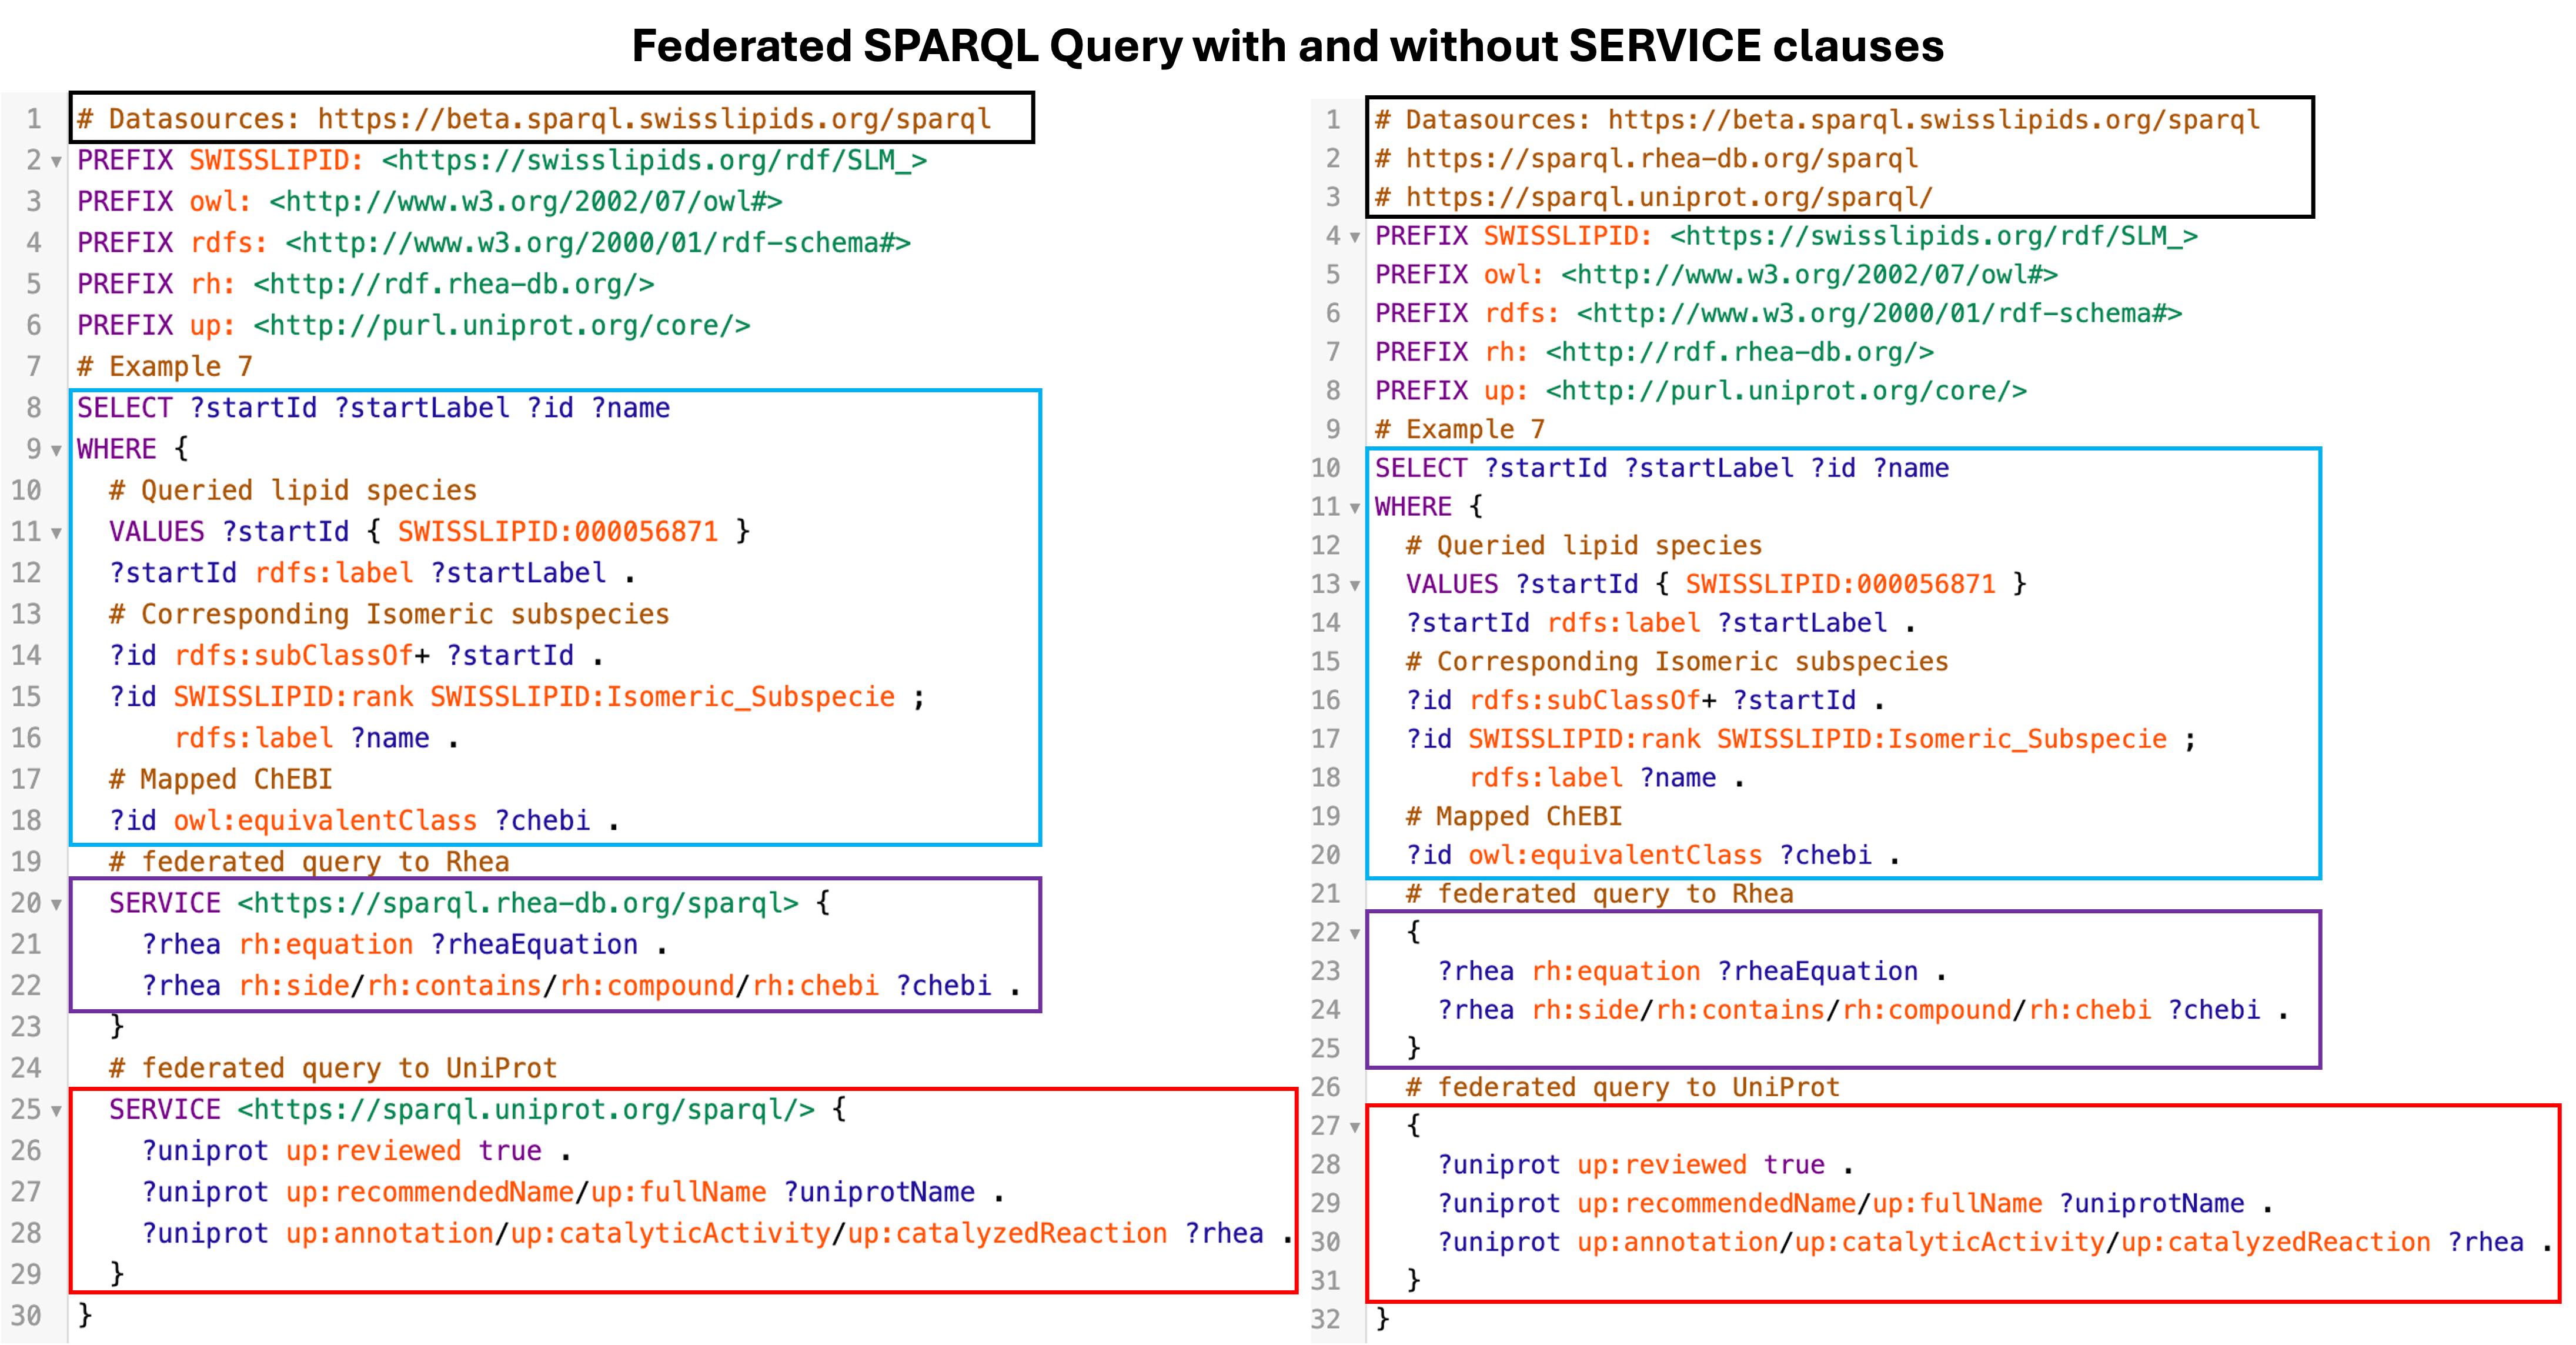
\includegraphics[width=1.0\textwidth]{query_content/sparql_query.png}
    \caption{
        Comparison of a federated SPARQL query manual server-side federation with \texttt{SERVICE} clauses (left) versus the equivalent query using client-side automated federation strategies without \texttt{SERVICE} clauses (right). Black box shows SPARQL endpoint URLs, Blue, Purple, and Red boxes designate sub-sections of the query sent to different endpoints.
    }
    \label{fig:sparqlQuery}
\end{figure}

\textbf{SPARQL} is the W3C-standard query language for retrieving and manipulating data stored in Resource Description Framework (RDF) format~\cite{Feigenbaum2013SPARQL}. 
\textbf{SPARQL federation} extends this model by enabling a single query to integrate the data of multiple, distributed data sources.
Figure~\ref{fig:sparqlQuery} displays two forms of a representative federated query (query \textit{7} in this study).

A crucial step in federated SPARQL query processing is \textit{source selection}: deciding which parts of a query are evaluated by which data sources. 
This can be specified \textit{manually} with the SPARQL 1.1 \texttt{SERVICE} keyword, as in the left panel of Figure~\ref{fig:sparqlQuery}, or handled \textit{automatically} by a client-side federation engine given only the query and target sources, as in the right panel. 
In both cases, \textit{query planning}, including join ordering, reducing intermediate results, and deciding whether joins are executed locally or at remote endpoints, also has a significant impact on overall query performance~\cite{Schmidt2010Foundations}. 
Automatic federation engines use different strategies for source selection, query partitioning, and optimization, and are further discussed in Section~\ref{sec3.1}.

The SPARQL query itself is a key factor in federated query performance. 
Even over a single endpoint, evaluation becomes more challenging as query structure grows in complexity and size.
In particular, the evaluation of basic graph patterns is known to be NP-complete, and the addition of operators such as \texttt{OPTIONAL} and \texttt{UNION} further increases evaluation complexity \cite{Perez2009Semantics}. 
Queries with many triple patterns can also produce large intermediate results and costly join operations, making planning and execution challenging~\cite{Schmidt2010Foundations}. 
In federated settings, these challenges are amplified: query engines must not only optimize joins and intermediate results locally, but also coordinate query decomposition, data transfer, and join execution across multiple remote endpoints with limited statistics and higher communication costs. 
Consequently, even moderately complex SPARQL algebra can become substantially harder to execute efficiently across multiple endpoints.


\section{Related Work}\label{sec3}
% Prior work largely studies algorithmic behavior under controlled conditions
Prior work on federated SPARQL querying has advanced algorithms for source selection, query planning, and distributed join processing, but has typically been evaluated under controlled benchmark conditions. 
While traditional, controlled benchmark settings yielded important insights into algorithmic efficiency, they provide a limited view of how federation behaves against public endpoints under dynamic real-world conditions. 
This study therefore, shifts the focus from stable benchmark environments to operational behavior in public settings.

\subsection{Federated Querying Algorithms}\label{sec3.1}
% SPARQL federation and common execution strategies
% FedX, SPLENDID, and source-selection/query-planning trade-offs
SPARQL federation has been studied primarily as a problem of \textit{source selection} and efficient intermediate-result processing. 
Systems such as \textsc{FedX} and \textsc{SPLENDID} illustrate two influential execution styles: \textsc{FedX} performs source selection dynamically at query time, avoiding reliance on precomputed source catalogs~\cite{schwarte2011fedx}, whereas \textsc{SPLENDID} uses standardized dataset metadata, in particular VoID descriptions~\cite{w3cvoid}, to guide source selection and planning~\cite{splendid2011}.
Other approaches target volatile environments, such as \textsc{ANAPSID}~\cite{anapsid2011}, or rely on custom statistics and metadata, including HiBISCuS~\cite{Saleem2014HiBISCuS}, CostFed~\cite{Saleem2018CostFed}, and FedUP~\cite{davat2024fedup}. 
From an endpoint maintainer’s perspective, however, publishing and maintaining such metadata is optional and often costly; consequently, endpoint-exposed metadata are often incomplete or unavailable in practice~\cite{Vandenbussche2017SPARQLES}. 
Federation is therefore commonly framed as query optimization under incomplete statistics and limited coordination between independently operated endpoints~\cite{montoya2017federation}. 
Given the real-world focus of our study, we evaluate only algorithms that do not depend on non-standard metadata for automated federation. Other relevant approaches, such as \textsc{ANAPSID}, were not included because no public implementations were available.

Recent systems have also made practical experimentation with federation strategies easier. 
In particular, \textsc{Comunica} provides a modular query engine in which source-selection methods, query planners, and join algorithms can be combined and compared~\cite{taelman2018comunica}. 
This modularity enables hybrid strategies, such as replacing \texttt{ASK}-based source selection, as used in \textsc{FedX}, with \texttt{COUNT}-based alternatives. 
Using a shared execution framework also reduces performance differences caused by implementation details, such as programming language, libraries, or threading models, allowing comparisons to focus more directly on the federation strategy itself.


\subsection{Federated Querying Benchmarks \& Evaluations}\label{sec3.2}
% Prior evaluations of SPARQL federation
% Public biological SPARQL endpoints as operational infrastructure
Benchmarks and empirical evaluations have played an important role in federated SPARQL research.
\textsc{FedBench} provides curated datasets and queries for comparing federation engines~\cite{Schmidt2011FedBench,Saleem2014FedBench}, while \textsc{LargeRDFBench} extends this approach to larger data volumes and more demanding federation scenarios~\cite{Saleem2018LargeRDFBench}. 
Other work has questioned how well curated or synthetic workloads capture the structure and difficulty of real query behavior, for example, in Wikidata-oriented benchmarking~\cite{Hernandez2015Wikidata}.

Although valuable for controlled comparison, these benchmarks typically assume stable execution environments and abstract away from operational characteristics of public SPARQL services, such as endpoint timeouts, rate limits, transient HTTP failures, changing metadata, and fluctuating responsiveness.
In real-world conditions, public endpoints can vary substantially in availability, interoperability, and performance~\cite{Vandenbussche2017SPARQLES}, and these factors can directly affect federated query execution, sometimes causing partial or complete failure.

Rather than proposing a new federation algorithm or benchmark suite, here we study how federated biological queries behave longitudinally over widely used public endpoints using three different federation strategies (one server-side and two client-side).
Our work therefore, complements prior algorithmic and benchmark-focused research by assessing the impact of real-world operational fragility, failure modes, and the gap between controlled benchmark assumptions and real-world use.


\section{Methods}\label{sec4}

\subsection{General Study Design}\label{sec4.1}
This study is a 13-month longitudinal evaluation of SPARQL query federation over public endpoints, focusing on the practical executability of real federated queries rather than controlled benchmark performance. 
Using the curated real-world query records described in Section~\ref{sec4.2}, we analyzed individual query executions within federation approach configuration--date experiments, enabling comparison across both federation approaches and changes in endpoint behavior over time. 
Because the evaluated strategies were implemented in \textsc{Comunica} rather than by directly invoking native \textsc{FedX} or \textsc{SPLENDID} binaries, we refer to them as \textit{metadata-free} (e.g., \textsc{FedX}) and \textit{metadata-guided} (e.g., \textsc{SPLENDID}) federation approaches throughout the study.
References to the companion results webpage are made throughout the paper as embedded links and direct to the same base webpage at the URL: \url{https://ecrum19.github.io/fed-survey-results/}.

\subsection{Real-World Queries}\label{sec4.2}
\textbf{Queries.}
The query corpus was obtained from users of SIB-hosted biological SPARQL endpoints~\cite{Bolleman2025sibqueries}. 
It contains 67 federated queries, all created by domain experts to answer real-world questions or test realistic scenarios. 
These queries were characterized in a structured CSV containing the original example query URL, natural-language description, target endpoint, federated endpoints, relevance/background notes, a ``toy'' flag, execution notes, similarity annotations, known problems, and aliases~\cite{fedSurveyResultsRepo}. 
The experimental repository stores the same corpus, with reduced metadata, in JSON format~\cite{fedSparqlSurveyExperimentsRepo}. 
More than half of the queries have a confirmed real-world application or address an open question, and around one quarter have produced results published in peer-reviewed papers.

To test client-side \textit{automatic} source selection, a preprocessing script~\cite{fedSparqlSurveyExperimentsRepo} generates two versions of each query: a \textsc{SERVICE} form, corresponding to the original query with one target source and explicit \texttt{SERVICE} clauses, and a \textsc{no-service} form, in which \texttt{SERVICE} clauses are removed, and multiple source targets are provided. 
Figure~\ref{fig:sparqlQuery} shows an example of both forms. 
We refer to experiments using the former as \textsc{SERVICE} experiments and those using the latter as \textsc{no-service} experiments.

All 67 queries were manually executed through the target endpoints' web interfaces to establish positive-control result sets for each query, reported in the \textit{service-control-31-03-2025-endpoint} experiment~\cite{fedSurveyResultsRepo}.

To characterize workload complexity, we extracted per-query features from the curated corpus, including triple-pattern counts, \texttt{OPTIONAL} and \texttt{UNION} usage, property paths, \texttt{DISTINCT}, \texttt{LIMIT}, and the number of federation members. 
Corpus-level summaries are available on the \href{https://ecrum19.github.io/fed-survey-results/}{companion results webpage}. 
Queries contain 14.90 triple patterns on average, ranging from 2 to 34, and involve an average of 2.24 federation members. 
About half use \texttt{DISTINCT} (mean 0.54), while \texttt{LIMIT} is less common (mean 0.18). 
Property paths appear frequently (mean 1.27), but recursive paths are less common (mean 0.49), suggesting that complex path recursion is concentrated in a subset of queries. 
Most queries contain no \texttt{OPTIONAL} or \texttt{UNION} clauses, with both averaging about 0.15 occurrences per query.
Figure~\ref{fig:complexityQuery}, available in a larger, interactive version on the \href{https://ecrum19.github.io/fed-survey-results/}{companion results webpage}, presents a per-query view of workload complexity by ordering queries by triple-pattern count and grouping them by the number of federation members.
Query features were extracted using a reproducible analysis script~\cite{queryAnalysisSibFederatedRepo}, and the full per-query feature table is available in the results repository~\cite{fedSurveyResultsRepo}.

Overall, the query set consists of moderately complex federated queries, typically spanning two or three sources, rather than simple joins over small fragments. 
At the same time, these queries are not dominated by advanced SPARQL features, suggesting that execution difficulty arises primarily from federation itself rather than from unusually complex query syntax.

\begin{figure}
    \centering
    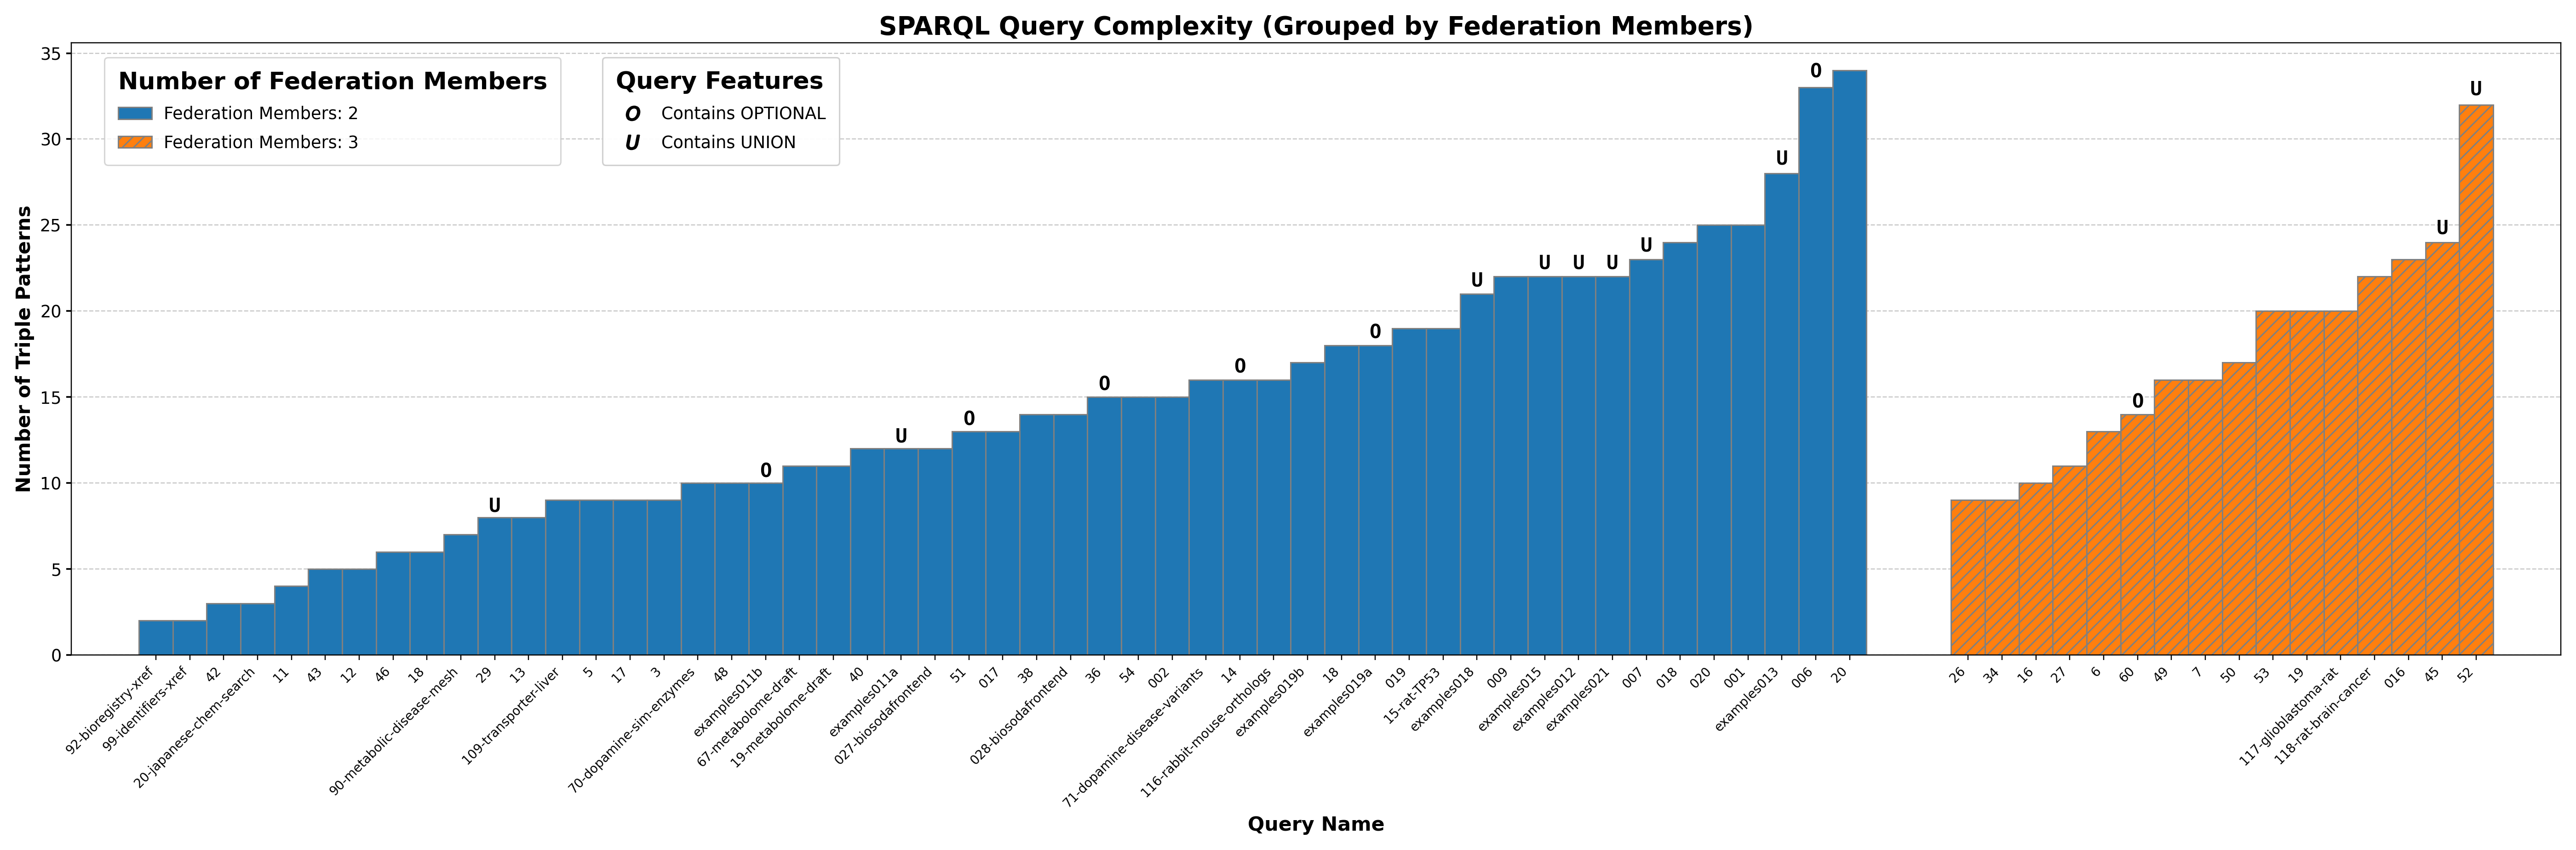
\includegraphics[width=1.0\textwidth]{query_content/Queries_Summary_Figure.png}
    \caption{
        Query complexity as a function of the number of triple patterns, federation members, and the presence of graph patterns. 
        More complex queries are those with OGPs, with a higher number of triple patterns and federation members, followed by those 
        with UGPs, following the same ordering in terms of triple patterns and federation members.
    }
    \label{fig:complexityQuery}
\end{figure}


Of the original 67 queries, 7 encountered errors early in experimentation and were excluded from \texttt{no-service} experiments.

\textbf{Endpoints.}
The workload involved seven \textit{target endpoints}, which receive complete \textsc{SERVICE} queries, and 14 \textit{federates-with endpoints}, which are contacted remotely through embedded \texttt{SERVICE} clauses. 
The complete endpoint list, URLs, descriptions, triple-stores~\cite{Erling2009VirtuosoRDF,bast2017qlever}, and citations is available on the \href{https://ecrum19.github.io/fed-survey-results/}{results webpage}. 
During the study, METRIN-KG replaced the earlier DBGI/EMI endpoint.
neXtProt~\cite{ZahnZabal2020neXtProt} was excluded from the study because its public endpoint was no longer maintained.


\subsection{Federation Approaches}\label{sec4.3}
The \textsc{Comunica} query engine framework~\cite{taelman2018comunica} v4.3.0 was used for both server-side manual federation (\textsc{SERVICE} experiments) and client-side automated federation (\textsc{no-service} experiments), while keeping the client-side execution environment constant. 
In \textsc{SERVICE} experiments, \textsc{Comunica} acts only as an external client: the complete query, including its explicit \texttt{SERVICE} clauses, is submitted to a single target endpoint, which is then responsible for federation tasks, carrying out remote requests, intermediate result joins, and returning the final results.
In contrast, in \textsc{no-service} experiments, with \texttt{SERVICE} clauses removed and multiple sources provided, \textsc{Comunica} performs client-side automated federation according to the predefined configuration.
Thus, the same engine is used in both settings, but automated federation is only performed in \textsc{no-service} experiments.

\begin{table}[t]
    \centering
    \scriptsize
    \caption{
        Comunica federation configurations used in our server-side automated federation experiments.
        A checkmark indicates the presence, while a dash indicates the absence of an approach within a configuration.
        \texttt{-NRL} variants disable client-side request rate limiting while leaving other configuration choices unchanged.
    }
    \label{tab:comunicaConfigs}

    \setlength{\tabcolsep}{3pt}
    \renewcommand{\arraystretch}{1.08}

    \begin{tabularx}{\linewidth}{Xccccc}
        \hline
        \textbf{Configuration}
            & \textbf{ASK}
            & \textbf{COUNT}
            & \textbf{VoID}
            & \textbf{Large est.}
            & \textbf{Rate limit} \\
        \hline

        \texttt{NOMETA-ASK}        & \checkmark & --         & --         & --         & \checkmark \\
        \texttt{NOMETA-COUNT}      & --         & \checkmark & --         & --         & \checkmark \\
        \texttt{VOID-TRIPLE}       & \checkmark & --         & \checkmark & --         & \checkmark \\
        \texttt{VOID-BLOCK}        & \checkmark & --         & \checkmark & \checkmark & \checkmark \\
        \texttt{-NRL}              & --         & --         & --         & --         & -- \\

        \hline
    \end{tabularx}
\end{table}

The client-side configurations in Table~\ref{tab:comunicaConfigs} isolate the main source-selection and planning assumptions tested in this study. 
\textsc{NOMETA-ASK} and \textsc{NOMETA-COUNT} rely on live endpoint probing, comparing lightweight source pruning against cardinality-oriented probing~\cite{schwarte2011fedx}. 
\textsc{VOID-TRIPLE} and \textsc{VOID-BLOCK} use available VoID descriptions and precomputed statistics at triple-pattern or larger query-block granularity~\cite{splendid2011,w3cvoid,hagedorn2014resource}. 
The \texttt{-NRL} variants disable client-side rate limiting without changing the underlying federation strategy. 
All configurations were applied through the experiment repository's \textsc{Comunica} configuration script~\cite{fedSparqlSurveyExperimentsRepo}.


\subsection{Experimental Set-up}\label{sec4.4}

\textbf{Observation period.}
The testing campaign comprised 20 experiments conducted between March 2025 and April 2026. 
We therefore treat the study as longitudinal, with repeated executions of the same workload and configuration families at multiple time points.

\textbf{Execution environment.}
Experiments ran on an Ubuntu 24.04.1 virtual machine with an Intel Core i5-9500 CPU (6 cores, 3.0 GHz), 64 GB RAM, a 468 GB NVMe SSD, and Linux kernel 6.8.0-45-generic. 
All queries targeted public endpoints, not local mirrors or replicated stores.

\textbf{\textsc{SERVICE} experiment workflow.}
In \textsc{SERVICE} experiments, queries were executed in their original form, preserving explicit \texttt{SERVICE} clauses and submitting the complete query to a single target endpoint. 
Each query was submitted with a single target endpoint as a datasource while retaining its embedded \texttt{SERVICE} clauses.

\textbf{\textsc{no-service} experiment workflow.}
The reproducible \textsc{no-service} workflow, documented in the study's experimental repository~\cite{fedSparqlSurveyExperimentsRepo}, follows four steps:
(1)\textsc{\seqsplit{query\_sort.py}}, (2)\textsc{\seqsplit{comunica\_configuration.py}}, 
(3)\textsc{\seqsplit{comunica\_run.py}}, and (4)\textsc{\seqsplit{localize\_results.sh}} \& \textsc{\seqsplit{organize\_data.py}}.
These correspond to query preparation, configuration selection, execution, and post-processing / summary generation, respectively. 
During execution, \texttt{\seqsplit{comunica\_run.py}} initializes a fresh \textsc{Comunica} engine instance via \texttt{\seqsplit{query-dynamic.js}} for each query executed. 
Datasources are read from the query header, SPARQL-JSON\cite{sparql11resultsjson} is requested as output, debug logging is enabled, and standard error is written to a per-query log file from which experiment-level summaries are generated. 

\textbf{Timeouts and retries.}
The execution script does not impose a wrapper-level wall-clock timeout, but does record wall-clock runtime from the logged start and end timestamps. 
Query termination is therefore determined by completion, endpoint-side failure, engine-level failure, or external process termination, and timeout-like phenomena are captured indirectly through these measured timestamps and failure modes. 
To reduce rate-limit effects, the execution script uses \texttt{--httpRetryCount=50} and inserts a one-second pause between queries if an HTTP-429 error~\cite{Nottingham2012RFC6585} is encountered.

\textbf{Endpoint request burden and error types.}
During experiments, we tracked the number of HTTP requests per query and the final error text or category when execution failed. 
These data support three operational metrics: endpoint request burden, endpoint-associated error rate, and failure-type distribution. 
In a longitudinal public-endpoint setting, these metrics help distinguish whether execution outcome changes stem from client-side federation planning, network or endpoint instability, or endpoint-side request handling.

\textbf{Definition of success and failure.}
An execution is considered to have \emph{produced results} if it returns parseable output conforming to the SPARQL 1.1 Query Results JSON Format~\cite{sparql11resultsjson}. 
Empty and non-empty result sets are distinguished using result count. 
Executions that produce no parseable output or terminate through an exception/error path are treated as explicit failures.
For the remainder of the study, we define \emph{execution success rate} as the proportion of executions that have produced a non-empty result set (i.e., result count > 0). 

\textbf{Result correctness and temporal reproducibility.}
This study does not verify semantic correctness of individual bindings, which would require complete local replicas of all participating endpoints. 
Instead, we use \textit{result-set size agreement} as a proxy: for each query, the reference size is the maximum result count observed under manual \textsc{SERVICE} execution, and later executions are considered consistent when they return the same count. 
Thus, ``correctness'' refers only to result-count agreement, not binding equality or semantic completeness. 
Temporal reproducibility is assessed by comparing identical query--configuration pairs across dated runs, including whether execution remained successful, whether non-empty results persisted, and whether error modes changed.


\section{Results}\label{sec5}
% Ground-truth control SERVICE experiments
We first compared the March 2025 \textsc{SERVICE} experiments to assess whether Comunica introduced systematic differences relative to direct endpoint execution.
Manual endpoint execution performed slightly better than the Comunica-mediated control, with higher \emph{execution success rates} (\(65.2\%\) vs. \(60.6\%\)) and fewer explicit errors (\(30.3\%\) vs. \(34.8\%\)).
However, the close agreement suggests that Comunica did not introduce a major confounding effect in subsequent experiments.

% General findings
An interactive all-query outcome heatmap, showing all experimental query executions chronologically, is available in the \textit{Overview Figures} section of the \href{https://ecrum19.github.io/fed-survey-results/}{results webpage}.

Overall, \textsc{SERVICE} experiments performed far better than \textsc{no-service} client-side automated federation experiments: \textsc{SERVICE} experiments had an \emph{execution success rate} of \(47.3\%\), and a \(46.2\%\) explicit error rate.
In contrast, \textsc{no-service} experiments had only a \(3.0\%\) \emph{execution success rate}, and \(95.1\%\) failed with explicit errors.
Thus, removing explicit \texttt{SERVICE} clauses and relying on automatic client-side federation reduced successful result production by roughly an order of magnitude and nearly doubled the error rate.
\textsc{no-service} experiments were also slower and more variable, with a median runtime of 4.47 seconds and a 90th percentile of 247.92 seconds, suggesting many failures involved severe slowdowns or stalled execution.


\subsection{Temporal Degradation of Query Success}\label{sec5.1}
% Discussion about decrease in efficacy over time ...
\begin{figure*}[t]
    \centering

    
\includegraphics[width=\textwidth]{Results/trend.png}

    \caption{
        The trend showing a decrease in the number of queries producing non-empty result sets in each run, grouped by experiment form.
        Explicit \texttt{SERVICE} control runs produced substantially more non-empty result sets than \texttt{no-service} runs, while later runs show a marked decline in successful result production.
    }
    \label{fig:queriesTrend}
\end{figure*}

Figure~\ref{fig:queriesTrend} illustrates the degradation of federated query success chronologically, showing that more queries obtained results in chronologically earlier executions for both \textsc{SERVICE} and \textsc{no-service} experiments.
For ease of comparison, we separated experimental executions into 4 distinct chronological groups: Spring 2025, Fall 2025, Winter 2026, and Spring 2026.
An in-depth, interactive data display of these time-based partitions can be viewed in the \textit{Monthly Views} section of the \href{https://ecrum19.github.io/fed-survey-results/}{results webpage}.

During Spring 2025, which included only \textsc{SERVICE} experiments, performance was strongest, with \(58.5\%\) \emph{execution success rate} and \(34.2\%\) explicit errors.
By Fall 2025, \emph{execution success rate} dropped to \(8.5\%\), explicit errors rose to \(85.9\%\), and runtimes became highly heavy-tailed, with the 90th percentile reaching approximately \(1.07\times 10^4\) seconds and a high HTTP request burden.
Winter and Spring 2026 remained low-success, high-error phases, with \emph{execution success rates} of \(2.1\%\) and \(2.7\%\), and error rates of \(96.7\%\) and \(96.5\%\), respectively.
Notably, the Spring 2026 \textsc{SERVICE} experiments also performed far worse than Spring 2025, with only \(14.9\%\) \emph{execution success rate}.
Although extreme runtime tails decreased by Spring 2026, successful result production did not recover.
Overall, Figure~\ref{fig:queriesTrend} shows this clear temporal decline in queries producing results.

Beginning in Fall 2025, many previously successful queries began failing after only 3--6 HTTP requests and roughly 4 seconds. 
Per-query logs show repeated \texttt{Server reported client-side error} events for \url{https://sparql.uniprot.org/sparql/}, with HTTP \texttt{403 Forbidden} errors, including for formerly stable queries such as \texttt{42}, \texttt{12}, and \texttt{16}. 
This indicates that server-side restrictions became a major contributor to the observed drop in success. 
According to the primary UniProt server administrator, this period coincided with increased AI-crawler traffic, including crawlers that ignored \texttt{robots.txt} guidelines discussed further in Section~\ref{sec6.2}.

Even when queries produced results, outputs were often unstable across repeated runs. 
Overall, 68.7\% of queries returned varying result counts, and 24 queries produced three or more distinct result-count outcomes. 
For example, \texttt{\seqsplit{92\_uniprot\_bioregistry\_iri\_translation}} returned 194 results in Fall 2025, later returned parseable but empty outputs, and eventually failed in Winter and Spring 2026. 
Thus, live federation can degrade not only through hard failures, but also through empty or otherwise reduced result sets.

\subsection{Explicit Error Taxonomy}\label{sec5.2}
% discuss the explicit errors observed and point to website for more details
Across experiments, failures clustered into recurring categories, visualized in the \textit{Query error-type heatmap by experiment run} on the \href{https://ecrum19.github.io/fed-survey-results/?mode=query&query=001&queryVariant=original}{results webpage}. 
The most frequent were \textsc{client-side HTTP} errors (n=577; 4xx endpoint rejections), \textsc{server-side HTTP} errors (n=222; 5xx failures), \textsc{transport-level} failures (n=85; incomplete responses such as \texttt{fetch failed}), \textsc{other} errors (n=80; e.g., HTTP 200 responses containing HTML error pages), and \textsc{timeout-related} errors (n=63). 
These failures reflect both endpoint-side constraints, including HTTP 403 rejections, server errors, malformed responses, and timeout-like interruptions, and client-side federation behavior, including large intermediate joins, heap exhaustion, and request explosion. 

\subsection{HTTP Requests and Queries that Obtain Results}\label{sec5.3}
% Talk about HTTP requests and outcome trends --> point to big HTTP request table
We examined whether successful \textsc{no-service} executions differed from failures in HTTP request burden, restricting the analysis to runs with valid request counts ($n=954$). 
Because request counts were highly skewed, we report both means and medians, and use permutation tests and Mann--Whitney U tests as assumption-light complements to correlation estimates~\cite{altman1994quartiles,good2005permutation,mann1947test}.

Under a broad success definition, any execution without an explicit error, successful runs issued more requests than failures on average (46{,}366 vs. 16{,}663) and by median (22 vs. 6). 
However, the association was weak ($r=0.049$), with only marginal permutation-test support ($p=0.065$ for correlation; $p=0.064$ for mean difference).
Using a stricter definition of success as a non-empty result set, successful executions again showed higher request burden, both in mean (68{,}085 vs. 16{,}560) and median (580 vs. 6). 
The effect remained small ($r=0.068$), but was statistically supported by permutation tests ($p=0.036$ for correlation; $p=0.033$ for mean difference) and by a Mann--Whitney U test ($p<10^{-6}$).

Overall, successful client-side automatic federation was not associated with fewer endpoint interactions. 
Non-empty results often required more HTTP activity, likely due to source probing, remote subquery execution, and intermediate-result transfer. 
However, small effect sizes and large mean--median gaps show that request burden was highly uneven and dominated by outliers, making HTTP request count alone a weak predictor of success. 
The most extreme HTTP request explosion cases issued hundreds of thousands to millions of HTTP requests before failing, examples include query \texttt{6} with 924{,}299 requests, query \texttt{13} with 742{,}417, and query \texttt{16} with 553{,}202 in experiment \texttt{NOMETA-ASK-17-9-25}.
Query- and experiment-specific plots are available in the \textit{Data Explorer} section of the \href{https://ecrum19.github.io/fed-survey-results/}{results webpage}.


\subsection{Comparison across federation approaches}\label{sec5.4}
Across the \textsc{no-service} experiments, all client-side automated federation algorithm families failed in most executions, with \emph{execution success rates} between only \(2.08\%\) and \(3.45\%\).
The corresponding counts were \(12/360\) for \textsc{NOMETA-ASK}, \(5/240\) for \textsc{NOMETA-COUNT}, \(6/180\) for \textsc{VOID-TRIPLE}, and \(6/174\) for \textsc{VOID-BLOCK}.
These results are visualized in the \textit{\textsc{no-service} algorithm efficacy comparison} graph on the \href{https://ecrum19.github.io/fed-survey-results/}{results webpage}.

Thus, all algorithms succeeded in a small minority of cases, but none were broadly robust for the tested workload. 
Differences between methods were modest: \texttt{VOID-TRIPLE} had the highest explicit-error-free rate, \texttt{VOID-BLOCK} the highest \emph{execution success rate}, and \texttt{NOMETA-COUNT} was consistently weakest. 
Success also varied substantially across runs, including multiple with \(0\%\) success, indicating general instability. 
Overall, VoID-based \textit{metadata-guided} strategies provided only a small advantage over \textit{metadata-free} strategies in \textsc{no-service} experiments.

The \texttt{-NRL} experiments show that client-side rate-limit mitigation did not seem to impact \emph{execution success rates}. 
Similar success ratios are observed for queries completed in Fall 2025 with and without rate-limit mitigation, and by Spring 2026, all configurations converged to complete failure. 
This suggests that client-side naive throttling or backoff cannot overcome tighter server-side policies.


\subsection{Unique Study Challenges and Endpoint Instability}\label{sec5.5}
A number of failures were caused by endpoint address changes outside the experiment’s control. 
Queries involving the former DBGI/EMI endpoint (14/67 queries) were affected by its migration to the production METRIN-KG endpoint URL. 
Similarly, \url{https://biosoda.unil.ch/emi/sparql}, a temporary federation server targeted in (14/67 queries), was deprecated in September 2025 and was removed from service in November 2025. 
These changes contributed to higher failure rates in Winter and Spring 2026 experimental runs.
For an in-depth view of endpoint-specific results by experiment, see the \textit{Endpoint outcomes by run} graph on the \href{https://ecrum19.github.io/fed-survey-results/}{results webpage}.

Although this complicates longitudinal interpretation, it reflects a central challenge of real-world SPARQL federation: queries depend on the continued availability, stability, and discoverability of independently maintained endpoints. 
When endpoints are moved, renamed, deprecated, or taken offline without redirects or client-interpretable explanations, users and engines typically observe only execution failure. 
Such changes are therefore not merely experimental noise, but examples of how federation breaks when endpoint-level compatibility is not preserved.



\section{Discussion}\label{sec6}

This study asks whether SPARQL federation works in the real world. 
We found that it can work in some cases, but it was not reliable for our complex biological query set over public endpoints.

\subsection{Manual and automated federation}\label{sec6.1}
Manual federation with explicit \texttt{SERVICE} clauses degraded substantially over the study period. 
Because the workload came from previously successful user queries, the Spring 2025 runs supported our expectation that many queries would remain executable. 
By Spring 2026, however, only 10 queries produced results, compared with more than 40 that did so consistently in Spring 2025. 
This decline reflects endpoint migrations, deprecations, and changing limit policies, showing that even manually specified federation can lose executability as independently maintained endpoints evolve.

Client-side automated federation was substantially more fragile and later became effectively non-viable. 
The fact that many of the same queries worked with explicit \texttt{SERVICE} clauses shows that the data and endpoints were not inherently unusable; failures arose when client-side engines had to infer source selection and plans under incomplete metadata, limited coordination, and public-service constraints. 
Two failure modes dominated: request explosion, where a single query produced hundreds of thousands of HTTP requests, and excessive local materialization, where large intermediate results exhausted client memory. 
From the endpoint perspective, such request-heavy plans can resemble abusive traffic; from the client perspective, they reveal planning assumptions that do not hold under live deployment constraints.

\subsection{Temporal instability and endpoint operations}\label{sec6.2}
SPARQL federation was not temporally consistent. 
Queries that succeeded at one time point later returned empty results or failed under the same client-side configuration, and Figure~\ref{fig:queriesTrend} shows a clear decline in execution success over time. 
Some change is expected in public infrastructure: datasets grow, endpoints move, backends change, and temporary services are deprecated. 
For example, during the study, UniProt had three data releases, grew by approximately 28 billion triples, and migrated from Virtuoso 7.2+ Open Source edition to QLever.  
Because of the backend changes, some UniProt queries to \url{https://sparql.api.identifiers.org/} began failing because the identifiers.org endpoint did not support the SPARQL protocol case where a query is sent as the body of a POST request.
These changes in public infrastructure pose challenges to federation but are feasible to remedy as discussed in Section~\ref{sec8}

A faster-moving challenge was observed in stricter server-side limits in response to bot and crawler traffic. 
According to the lead UniProt server administrator, UniProt's SPARQL endpoint historically saw tens to hundreds of thousands of visitors per month between 2020 and 2024, but in Summer 2025, some months exceeded three million visitors, without a comparable increase in hardware. 
Traffic remained around five times higher than the 2024 baseline in 2026. 
UniProt therefore tightened limits on response time, concurrent queries per IP, request rates, and daily request volume. 
For federation, the main problem is that such limits, migrations, and deprecations are rarely communicated in machine-readable ways that client engines can interpret; users often see only failure and errors.

\subsection{Implications for real-world federation}\label{sec6.3}

Public biological SPARQL endpoints are shared research infrastructure, typically optimized for interactive exploration, documented examples, and moderate programmatic access. 
This creates a mismatch with automated federation: a single user query can be decomposed into many rapid requests, large intermediate transfers, or long-running connections. 
As a result, an endpoint may be reliable for single-endpoint use while still being poorly suited to unrestricted cross-endpoint federation.

This mismatch also limits what controlled benchmarks can show. 
Benchmarks remain valuable for isolating algorithmic effects, but they can overestimate real-world viability when they abstract away from endpoint instability, incomplete metadata, request policing, backend changes, cache behavior, public-service load, and temporal drift. 
Practical federation therefore, requires more research into cooperation between servers and clients. 
Endpoint providers should invest in clearer operational metadata, migration signals, and machine-readable limits, while client-side engines should integrate request budgets, endpoint-aware planning, adaptive backoff, diagnostics, and safeguards against request explosion.

For heavier workloads, algorithmic improvements alone may not be sufficient. 
More sustainable architectures, such as negotiated access, mirrors, caches, precomputed source summaries, controlled federation gateways, or hybrid deployments, may be necessary. 
The main lesson is not that SPARQL federation is impossible, but that open-ended federation over public endpoints should not be assumed to be operationally sustainable by default.

\section{Limitations}\label{sec7}
This study has three main limitations. 
First, it is domain-specific: the workload and endpoints come from the biological Linked Data ecosystem and should not be generalized automatically to all SPARQL federation settings. 
Second, the corpus contains 67 real-world queries over a limited set of public endpoints, which is meaningful but not exhaustive. 
Third, changing endpoint behavior makes causal attribution difficult; the artifacts show when outcomes changed, but not always the precise administrative or infrastructural cause.

\section{Practical Implications and Recommendations}\label{sec8}
This study examines a demanding but high-value use case: complex biological federation over authoritative public resources maintained by communities that recognize its scientific value. 
The results do not disprove federation for simpler settings, but they show that current algorithms, protocols, and infrastructure are not robust enough for this realistic workload.

The practical priority is to make federation more operationally aware. 
Researchers should evaluate algorithms longitudinally over public or public-like endpoints, reporting not only runtime and result counts but also failure modes, temporal reproducibility, and request burden. 
Engine developers should investigate adding request budgets, rate-limit-aware planning, adaptive backoff, result caching, and actionable diagnostics. 
Endpoint maintainers should expose machine-readable limits, retry behavior, redirects, supported request forms, pagination expectations, and service status. 
For workloads beyond what public interactive endpoints can sustainably support, controlled federation gateways, negotiated access, mirrors, shared caches, precomputed source summaries, or low-cost publishing approaches such as Triple Pattern Fragments~\cite{Verborgh2016TPF} may be needed.


\section{Conclusion}\label{sec9}
This study presented an in-use evaluation of SPARQL federation over large public biological endpoints, using real-world federated queries and multiple client-side federation strategies. 
We broadly assessed the question: "Does SPARQL federation work in the real world?"
Generally, we found that execution success declined sharply over time, as public endpoints changed and tightened limits that client-side federation engines could not adapt to.

The main lesson is that SPARQL federation is not only an algorithmic problem, but an operational one. 
Even when the data exist and the queries are meaningful, successful execution depends on the alignment of query planning, endpoint availability, metadata, rate limits, backend behavior, and network reliability. 
When that alignment breaks, federation fails not as a Semantic Web principle, but as a practical workflow: queries return errors, empty outputs, or unstable results.

SPARQL federation remains conceptually powerful, but dependable live federation over public endpoints cannot be assumed. 
Without federation-aware infrastructure, clearer endpoint policies, better diagnostics, and planners designed for public-service constraints, distributed Knowledge Graphs risk remaining theoretically linked but operationally difficult to integrate.


%\begin{credits}
%\subsubsection{\ackname} 
%Project funding provided from the Research Foundation – Flanders (FWO) (SB Fellowship 1S27825N) and (Long Research Stay V416635N).
% Ruben Taelman is a postdoctoral fellow of the Research Foundation – Flanders (FWO) (1202124N).
% Tarcisio Mendes acknowledge support from the Swiss National Science Foundation through the MetaboLinkAI project (10.002.786).
% \end{credits}

\section*{Declaration on Generative AI}
The authors used ChatGPT-5.5 (OpenAI) to assist with grammar suggestions, spell-checking, LaTeX and BibTeX formatting, and create the result webpage\cite{fedSurveyResultsRepo} during manuscript preparation. 
The tool was not used to generate research data, perform experiments, conduct statistical analyses, or draw scientific conclusions. 
All AI-assisted text was reviewed, edited, and approved by the authors, who take full responsibility for the content of the manuscript.

\bibliographystyle{splncs04}
\bibliography{references}

\end{document}
